\chapter{CODE VERIFICATION}
\label{chap:model_analysis}
The algorithms described in this chapter are implemented in Fortran, with source code listed in Appendix \ref{chap:fortran} and available online.
The correctness of the implementations is verified in Chapter \ref{chap:model_analysis}, and their performance is subsequently analyzed.

% TODO: Revise
In this chapter, both numerical implementations of the model are probed.
We begin by verifying that the methods are mistake-free by looking at convergence orders.
Then, the two methods are compared, to determine the conditions under which the asymptotic
approximation is valid.
Finally, results are compared to simpler kelp models.

\section{Confidence Building in Computational Codes}
%TODO: Citations
As Roache explains, there are two aspects to confidence building for numerical codes, specifically those which solve PDEs:
verification deals with \textit{solving the equations right}, while validation deals with \textit{solving the right equations}.
Validation involves comparison with experimental evidence in order to determine that governing equations
accurately describe physical phenomenon, and that their solutions match observation.
Validation is an ongoing process.
As new experimental data becomes available, the equations can be solved in an attempt to replicate the observation.
Verification, however, is a purely mathematical exercise, and has nothing to do with the physical system being modeled.
It deals only with the agreement between an equation and its numerical solution produced by a particular implementation of an algorithm.
Unlike validation, verification is something to be started and finished.
If a set of parameters to the model can be chosen to exercise all terms in the equation, comparison between the numerical and exact solution is sufficient to demonstrate the correctness of a computational code, and the process need not be repeated unless the code is modified.

Due to lack of sufficient experimental data, rigorous validation of the model is left as future work.
However, verification of both the finite difference and numerical asymptotics algorithms is presented here.
There are two forms of verification.
The first is \textit{verification of codes}, where a whole implementation of an algorithm is tested, and the the difference between the numerical and analytical solutions is \textit{explicitly measured} at every point in the numerical solution.
The same calculation is repeated for several grid sizes, and it is checked that the convergence order as the grid spacing approaches zero matches the theoretical convergence order of the algorithm.
The explicit measurement of errors requires that the analytical solution be known, which is generally only possible for some unrealistic or uninteresting set of parameters.
If the analytical solution were available for the real, interesting case, then it would probably not have been necessary to implement a numerical solution in the first place.

Therefore, the second phase of verification is \textit{verification of calculations}, where a single specific calculation is performed, and the error is \textit{estimated} since it cannot be measured explicitly.
This is generally done by repeating the calculation for several grid sizes, as above, then using a technique called \textit{Richardson Extrapolation} to estimate the limiting solution as the grid spacing approaches zero.
This estimated limiting solution is then compared to the actual numerical solutions.
Error estimation for a specific calculation can be used to calculate error bars to display on a plot to represent discretization error in the solution.

\section{Code Verification: Method of Manufactured Solutions}

The most obvious way to obtain an analytical solution to compare to a numerical solution is by choosing a simple case where the PDE can be solved explicitly, perhaps through separation of variables or by reducing it to an ODE.
This is referred to as the Method of Exact Solutions.
However, such simple cases usually result in such a loss of generality that they become useless in testing the complicated aspects of the solution algorithm.
In order to verify that a code will work in an interesting case, every term in the equation must be exercised during the verification process.
An alternative process, the Method of Manufactured Solutions, retains arbitrary generality in the equations while making analytical solutions readily available.
Of course, there is a trade-off: the solutions are not physically realistic.
However, this is not an issue.
As stated previously, \textit{verification is a purely mathematical endeavor}.
Determining that a code solves an equation correctly is unrelated to physical realism.

Consider a differential equation
\begin{align}
  Du(\vec{x}) = \sigma(\vec{x}), \label{eqn:mms_de} \\
  u(\vec{x})=f(\vec{x}) \mbox{ for } \vec{x} \in \Sigma,
  \label{eqn:mms_bc}
\end{align}
where $D$ is a differential operator, $u$ is the solution, $\sigma$ is a source term, $f$ is the boundary condition function, and $\Sigma$ is the set of boundary points at which the boundary condition is applied.
In general, $D$, $\sigma$, and $f$ are known, and solving for $u$ involves determining $D^{-1}$ and calculating $u = D^{-1}\sigma$ while satisfying \eqref{eqn:mms_bc}.

The Method of Manufactured Solutions reverses the normal procedure.
Here, $u$ is hand-picked at the outset, all parameters and coefficient functions in $D$ are chosen to be nonzero, and the source term $\sigma$ which produces the desired solution is calculated.
Similarly, the boundary condition is determined from the chosen solution.
In essence, rather than solving $u = D^{-1}\sigma$ subject to $u=f$, it suffices to compute $\sigma = Du$ and evaluate $f=u$ at the boundary.
Whereas \textit{inverting} a differential operator analytically is impossible for many equations and often requires ingenuity when it is, \textit{applying} one is a plug-and-chug application of algebra and calculus.
Of course, it is necessary to construct $u$ and any coefficient functions in $D$ from simple, differentiable and integrable functions.

Also, $u$ must satisfy any constraints imposed by the algorithm such as hard-coded boundary conditions or requirements for positive coefficients.
Finally, the chosen functions should have small derivatives so that convergence can be achieved for reasonable grid sizes.
Since these functions may need to be fairly complicated in order to achieve full generality while meeting the necessary constraints, it is advisable to use a \textit{Computer Algebra System} (CAS) to perform the symbolic manipulations involved in computing $\sigma$.

\subsection{Symbolic Variables and Solution}
In order to verify the numerical implementations described in the previous chapters, it is necessary to first choose a manufactured solution $L(\vec{x}, \vec{\omega})$ to the radiative transfer equation, as well as coefficient functions for the absorption coefficient $a(\vec{x})$ and volume scattering function $\beta(\vec{\omega}\cdot\vec{\omega'})$.
For the particular implementations developed in this thesis, the following conditions must be met by the manufactured solution:
\begin{enumerate}
  \item Periodic solution and absorption coefficient in $x$ and $y$
  \item Positive solution and absorption coefficient
  \item Position-independent surface downwelling boundary condition
  \item Zero upwelling radiance at the bottom boundary
  \item Properly normalized VSF $\beta(\Delta)$, as described in Section \ref{sec:iops}
\end{enumerate}


% TODO: Revise
\subsection{Finite Difference}

% TODO: Discuss OAMs (order of accuracy mistakes)
The only source of error in the finite difference method is discretization error due to the truncation of terms in the Taylor Series during the construction of the finite difference formulas in Section \ref{sec:discretization}.
Each of the derivatives in this implementation are approximated by two terms in the Taylor series: the leading order and first order terms.
Therefore, the error should be second order in grid spacing.
That is, when the grid spacing is sufficiently small, decreasing it further should result in the discretization error approaching zero quadratically.
Of course, if large grid spacings are used, then quadratic convergence may not be observed even in a correct implementation since higher order terms in the Taylor series error will dominate the quadratic term.
But for small grid spacings, the second order term dominates.
The range of small grid spacings for which the lowest order term dominates is known as the \textit{asymptotic range}.
% TODO: revise.
Whenever verification is performed, it is essential that the asymptotic range is achieved, either by using finer grids or using a solution and variable coefficients with smaller derivatives.
% TODO: Discuss what MMS verifies.
% TODO: Move to overview section, not FD specifically?
% TODO: Big Oh notation (1D)
% TODO: Big Oh doesn't carry over to multiple dimensions

In the particular case of the radiative transfer equation in three spatial dimensions,
there are five discretized variables $(x,y,x,\theta,\phi)$.
A five dimensional resolution space is nontrivial to characterize, so we define generic spatial and angular resolutions for the sake of reducing dimensionality,
Let $n_s = n_x = n_y = n_z$ and $n_a = n_\theta = n_\phi$.
Then, we use the geometric mean to describe the spatial and angular resolution, as
\begin{align}
  ds &= (dx\, dy\, dz)^{1/3}, \\
  da &= (d\theta\, d\phi)^{1/3}.
\end{align}

This reduces the dimenionality of the resolution space to two, but big oh convergence is really only well-defined for a single variable.
Therefore, the finite difference verification is performed by holding $n_a=8$, and varying $n_s$ between 4 and 64.
As shown in Figure \ref{fig:fd_mms}, second order convergence is observed, demonstrating that the code works without order-of-accuracy mistakes.
% TODO: Discuss multidimensional error further
% TODO: Discuss log-log plot.

\begin{figure}[H]
  \centering
  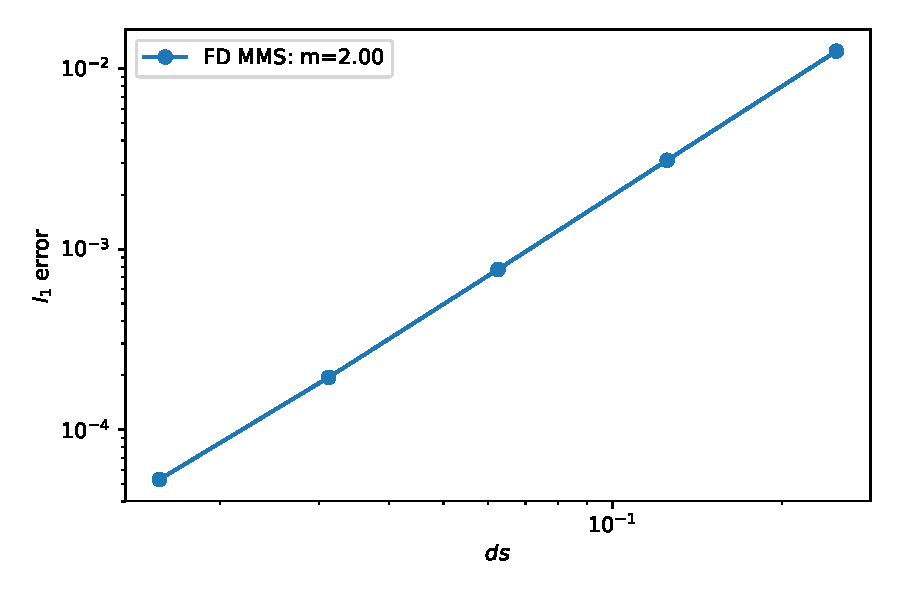
\includegraphics[width=5in]{fd_mms}
  \caption{Code verification for the finite difference solution via the Method of Manufactured Solutions. Each point represents the same simulation run with a different spatial grid sizes, with the angular grid held constant at $n_a=8$. The average absolute difference between the analytical and numerical solutions is shown. A slope of $m=2$ on a log-log scale demonstrates second order convergence, as expected. This demonstrates the correctness of the code.}
  \label{fig:fd_mms}
\end{figure}

\begin{figure}[H]
  \centering
  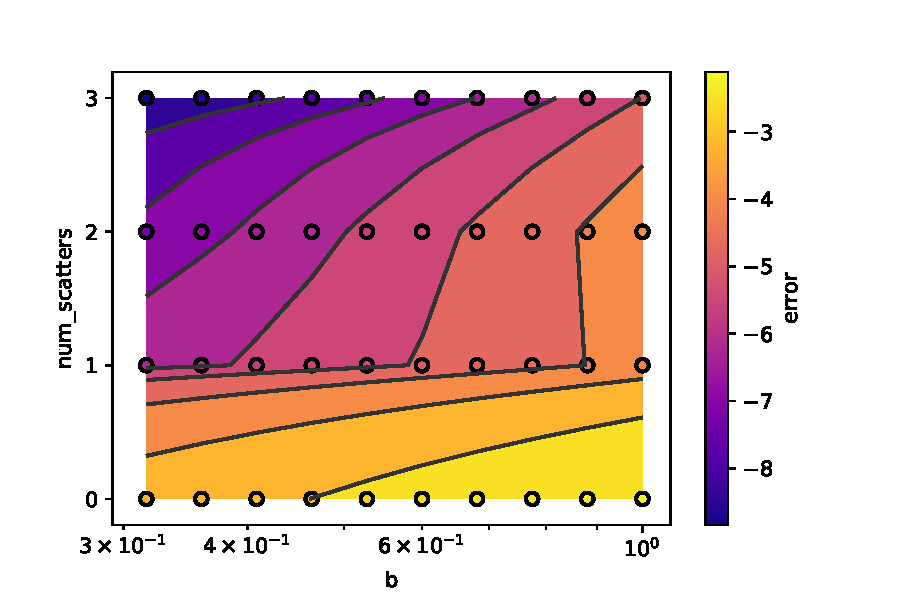
\includegraphics[width=5in]{mms_asym_err_n_contourf}
  \caption{mms asym n contourf}
  \label{fig:mms_asym_err_n_contourf}
\end{figure}

The quantity that we compare is \textit{perceived irradiance}, which is different than the simple mean irradiance in each depth layer.
Rather, the average is weighted by the normalized spatial kelp distribution to determine the average irradiance experienced by the kelp population.
For more detail, see Section \ref{sec:perceived_irrad}

% TODO: Revise
In varying $n_s$, we see that the accuracy is very low for small $n_s$ values.
This is because in these cases, the horizontal grid cells are too large to capture any detail
about the kelp fronds near the bottom where they are very small.
The kelp is effectively not present in these layers, and therefore the perceived irradiance is zero.
After increasing the resolution past this minimum threshold, however, little improvement results

% TODO: Revise
\subsection{Numerical Asymptotics}

In the first two cases, when the scattering coefficient is the same order or smaller as the absorption coefficient,
the asymptotic approximation converges to the finite difference solution.
However, in the very turbid water of the San Diego Harbor, the scattering coefficient is an order of magnitude higher
than the absorption coefficient, causing the asymptotic solution to quickly diverge.
In figure \ref{fig:asym_conv_compare}, average relative errors for the two converging cases are shown.
In both cases, the accuracy improves with more scattering events until it plateaus.
In the first case, 4 scattering events is sufficient, whereas in the second, the accuracy improves until 12 scattering events.

\begin{figure}[H]
  \centering
  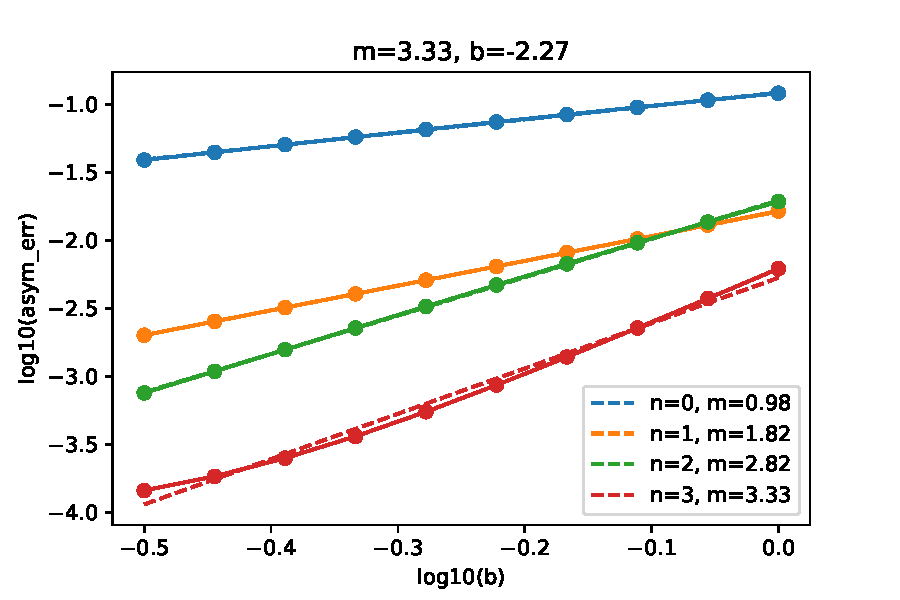
\includegraphics[width=5in]{mms_asym_b_conv}
  \caption{Code verification for the numerical asymptotics solution via the Method of Manufactured Solutions. A range of $b$-values are run, using 0 - 3 terms in the asymptotic series. Ideally, the $n-th$ order approximation should demonstrate $n+1$-th order convergence as $b \to 0$. The first three approximations are reasonably close, but the $n=3$ approximation converges slower than expected. It is unclear whether this is due to a coding mistake, discretization error, or if there is another cause for the sub-optimal convergence.}
  \label{fig:mms_asym_b_conv}
\end{figure}

\section{Verification of Calculations}
% TODO: Intro
\subsection{Richardson Extrapolation}
Richardson extrapolation, is a technique for estimating the continuum value of a scalar functional derived from a solution to a differential equation by using values of the scalar obtained from numerical solutions on several different grids.
The technique was developed by Richardson in 1912 with an application paper related to a stresses on a dam, and is also known as $h^2$ extrapolation since it was originally applied to a second order method.

Let the scalar of interest be called $\phi$ and the grid spacing $h$.
Denote the exact solution as
\begin{equation}
  \phi_e = \lim_{h \to 0} \phi(h),
\end{equation}

The crux of the technique is to assume that discretization error can be written as a linear combination of powers of $h$, as in a Taylor series.
That is,
\begin{equation}
  \phi - \phi_e = g_0 + g_1 h + g_2 h^2 + g_3 h^3 + \cdots.
\end{equation}
Assuming that a second order numerical method is used, the first two terms on the right hand side are zero.
For a first order method, only the first term is necessarily zero.
Of course, in a ``zeroth order'' method, the absolute error is bounded from below by $|g_0|$, and so does not approach zero as the grid is refined.
``Zeroth order'' methods are also known as ``incorrect.''

The original techniques involves numerical solutions on two grids with spacings $h_1 < h_2$ (i.e., grid 1 is finer), from which scalars $\phi_1$ and $\phi_2$ are calculated respectively.
The ratio $r = h_2/h_1$ is called the grid refinement ratio.

Then,
\begin{align*}
  \phi_1 &= \phi_e + g_2 h_1^2 + O(h^3), \\
  \phi_2 &= \phi_e + g_2 h_2^2 + O(h^3).
\end{align*}
Solving for $g_2$ yields
\begin{equation*}
  g_2 = \frac{\phi_1 - \phi_e}{h_1^2} + O(h^3), \\
\end{equation*}
so
\begin{align*}
  \phi_1 &= \phi_e + \frac{h_2^2}{h_1^2}(\phi_1 - \phi_e) + O(h^3) \\
  &=  \phi_e + r^2(\phi_1 - \phi_e) + O(h^3) \\
  &= \phi_e(1-r^2) + \phi_1 r^2 + O(h^3). \\
\end{align*}
Hence, the approximate continuum solution is
\begin{equation*}
  \phi_e = \frac{\phi_2 - \phi_1 r^2}{1 - r^2} + O(h^3).
\end{equation*}
In essence, Richardson extrapolation allows for $\phi$ values from two solutions of order $h^p$ to be combined to produce an approximation of order $h^{p+1}$ to the continuum value of $\phi$.

\subsection{Generalized Richardson Extrapolation}
Of course, the above equations are only approximations.
In reality, higher order terms introduce noise which may distort the extrapolated value
when only two grid sizes are used.
In order to reduce this noise, the concept can be easily generalized to incorporate more than two numerical solutions, as follows.
From
\begin{equation*}
  \phi \approx \phi_e + g_2 h^2,
\end{equation*}
it is clear that $\phi$ is approximately linear in $h^2$.
Therefore, a simple linear fit through multiple points in $(h^2, \phi)$ space yields $\phi_e$ as the y-intercept.
The slope, $g_2$, can be discarded.
If significant noise due to outliers still distorts the extrapolated values during fitting, a robust fitting algorithm such as Huber \cite{yu_robust_2014} or Ridge \cite{hoerl_ridge_1970} regression can help reduce the influence of outliers.

Additionally, this take on Richardson extrapolation is trivially applied to multiple dimenisions.
For a grid which has several resolution parameters $h_1, h_2, \ldots, h_n$ (e.g. multiple spatial dimensions, or spatial and angular grid resolutions), if the algorithm is second-order in each resolution parameter, then
\begin{equation*}
  \phi \approx \phi_e + g_{21} h_1^2 + g_{22} h_2^2 + \ldots + g_{2n} h_n^2.
\end{equation*}
Hence, fitting a plane or hyper-plane through several points in $(h_1^2, h_2^2, \ldots, h_n^2, \phi)$ space similarly produces $\phi_e$ as the y-intercept.
